\chapter{Background}
\label{chap:background}

In this chapter we provide some background on the MDP framework, which is the representation of the problem used by our algorithms to obtain agent policies. We then describe reinforcement learning and the basic policy iteration algorithm, followed by a discussion of GPU architectures and general purpose programming on the GPU.

\section{Markov Decision Process}

A \emph{Markov Decision Process} (MDP) \cite{norvig} is a specification of a sequential decision process in a fully observable environment with five components. An MDP can be represented by the 5-tuple $(\mathcal{S, A, P}, R, \gamma)$ where: $\mathcal{S} = \{s_1, s_2, ..., s_n\}$ is a finite set of states; $\mathcal{A} = \{a_1, a_2, ..., a_m\}$ is a finite set of actions; $\mathcal{P}$ is a Markovian transition model where $\mathcal{P}(s, a, s')$ is the probability of making a transition to state $s'$ when taking action $a$ while in state $s$; $R$ is a reward function such that $R(s, a, s')$ is the reward for the transition represented by $(s, a, s')$; and $\gamma \in [0, 1)$ is a discount factor for future rewards.

The solution to an MDP is a \emph{policy}, denoted by $\pi$. Given the stochastic nature of an MDP, a given policy is rated based on the expected utility, as measured by $R$, of actions selected by the policy. The optimal policy for a given MDP is the policy which yields the highest expected utility and is denoted by $\pi^*$. An agent following policy $\pi^*$ acts by determining the current state $s$, and executing the action specified by $\pi^*(s)$.

When defining the expected utility of an MDP, the horizon must first be described as finite or infinite. A finite horizon occurs when there is a fixed time $N$ after which actions have no effect on reward or cost. An infinite horizon does not have any fixed limitation. With an infinite horizon the optimal policy is stationary; that is, $\pi^*(s)$ is independent of time. With a finite horizon the optimal policy changes over time and is described as non-stationary. We assume all MDPs have an infinite horizon.

Given an MDP with infinite horizon the utility of a state sequence can be defined as either additive or discounted. For additive rewards the utility of a state sequence is:
\[
    U_h([(s_0,a_0),(s_1,a_1),(s_2,a_2),...]) = R(s_0,a_0,s_1) + R(s_1,a_1,s_2) + R(s_2,a_2,s_3) + ...
\]
For discounted rewards the utility of a state sequence is:
\[
    U_h([(s_0,a_0),(s_1,a_1),(s_2,a_2),...]) = R(s_0,a_0,s_1) + \gamma R(s_1,a_1,s_2) + \gamma^2 R(s_2,a_2,s_3) + ...
\]
The discount factor $\gamma$ is defined as a number between $0$ and $1$. From this it is clear that additive rewards is a special case of discounted rewards with $\gamma = 1$.  Note that as $\gamma$ approaches $0$, the utility function becomes weighted toward immediate rewards and as $\gamma$ approaches $1$ the utility function becomes weighted toward long term rewards. We assume all MDPs use discounted rewards with $\gamma \in [0, 1)$.

\section{Policy Iteration}

Given a complete model, $(\mathcal{S, A, P}, R, \gamma)$, of an MDP it is possible to use the policy iteration algorithm to determine an optimal policy. The policy iteration algorithm requires some initial policy $\pi_0$ followed by the repeated iteration of two steps: policy evaluation and policy improvement \cite{norvig}. Policy evaluation calculates the utility of policy $\pi_i$ such that $U^{\pi_i} = U_i$ where 
\[
    U^{\pi_i} = R(s_0,\pi(s_0)) + \gamma R(s_1,\pi(s_1)) + ...
\] 
Policy improvement computes a new policy based on $U_i$ in an attempt to improve on policy $\pi_i$. These two steps are repeated until the policy improvement step no longer yields a change in the utilities: $U_i \approx U_{i+1}$.

To confirm that this results in an optimal policy, we must examine how the utility function is generated during each iteration. For compact notation let $R(s,a)$ be the weighted sum of rewards over $s'$:
\[
    R(s,a) = \sum_{s' \in S} \mathcal{P}(s,a,s')R(s,a,s')
\]
Assuming the goal is to maximize the utility, the optimal policy can be defined using Equation \ref{eq:opt:policy}.
\begin{equation}
    \pi^*(s) = \argmax_a \sum_{s'} \mathcal{P}(s,a,s')U^*(s')
    \label{eq:opt:policy}
\end{equation}

The maximum utility of a state satisfies the Bellman optimality criterion:
\[
    U^*(s) = R(s,a) + \gamma \max_a \sum_{s'}\mathcal{P}(s,a,s')U^*(s')
\]
This function is derived from the idea that the utility of each state is equivalent to the reward at that state plus the sum of the discounted rewards of all following states. For an MDP with $n$ states there are $n$ Bellman equations and $n$ unknowns (the utilities of the states). Optimizing the Bellman criterion provides an optimal policy. One way to do this is to use dynamic programming and the Bellman update:

\begin{equation}
    U_{i+1}(s) \gets R(s,a) + \gamma \max_a \sum_{s'}\mathcal{P}(s,a,s')U_i(s')
    \label{eq:bellman:update}
\end{equation}

The utility function $U_i$ which results from policy iteration is a fixed point of the Bellman update, which means it is a solution to the Bellman optimality criterion and thus $\pi_i$ must be an optimal policy.

To perform the policy evaluation step we can use the Bellman equation:
\begin{equation}
    U_i(s) = R(s,a) + \gamma \sum_{s'} \mathcal{P}(s, \pi_i(s), s')U_i(s')
    \label{eq:bellman:eval}
\end{equation}

The optimal policy can now be determined using Equation \ref{eq:bellman:eval} to determine $U_i(s)$ for all $s \in S$ and using Equation \ref{eq:bellman:update} to generate $\pi_{i+1}(s)$.

\section{Reinforcement Learning}

Policy iteration requires the complete model of the underlying MDP. However, in practical control problems it is often the case that a complete model is not available \cite{lspi}. Most commonly, the transition model and reward function are unknown. To solve these problems we need agents which can learn optimal policies through the process of reinforcement learning. A typical reinforcement agent will generate a policy by acting within the environment and use positive and negative outcomes to reinforce good policy decisions and avoid bad policy decisions.

The observations of an agent acting in an environment can be organized in tuples referred to as samples: $(s, a, r, s')$. This sample layout means the agent was in state $s$, took action $a$, received reward $r$, and ended up in state $s'$. These samples can be collected by interacting with the environment or by using a simulation of the environment.

\subsection{Online and Offline Reinforcement Learning}

An online reinforcement learning agent is one which performs policy updates while actively interacting with the environment. A typical online reinforcement learning agent will start with some initial policy and interact with the environment by either selecting an action at random or following the current policy. The proportion of time the agent spends randomly selecting an action is the exploration rate. Changing the exploration rate will affect the policy generated by shifting toward or away from local maximums. An agent with a very low exploration rate is likely to generate a policy based on the earliest successful actions it takes, while an agent with a very high exploration rate may take longer to converge to a policy but is more likely to explore the entirety of the state-space. Some agents use more advanced exploration policies in an attempt to explore the state-space more effectively.

In contrast, an offline reinforcement learning agent generates a policy without directly interacting with the environment. Generally this is achieved by using existing samples from the environment or a simulation. Because offline agents do not directly interact with the environment they do not have control over exploration policy in the environment. This can be limiting; however, this also provides a high level of flexibility as there are no restriction on how the samples are gathered. For example, an offline agent can trivially generate a policy based on the experience of an existing agent or even multiple existing agents. With online agents this is usually not possible, although an existing online agent can provide a starting policy for another agent.

A key benefit of offline agents is the decoupling of action selection and policy updates. As a result, offline algorithms generally guarantee convergence in the presence of approximate models. In addition, decoupling the action selection from policy updates reduces the number of operations necessary for an agent to make decisions. 

In video games action selection decoupling is particularly important as agents have a very strict time restrictions. Video game agents are expected to act at least as often as graphics are drawn to the screen. Using a minimum framerate of 30 hertz results in a maximum decision time of 33 ms \cite{game:ai:lecture}. When an online agent selects an action, it is also required to perform a policy update step. Because of this requirement it may be unfeasible to use online agents in a video game; however, an offline agent may be more feasible because the policy update step is decoupled from interacting with the environment.

\section{General Purpose Programming on the GPU}

In the early 1990s the central processing unit (CPU) was responsible for almost the entirety of processing on a desktop computer system, including the video output. Following the advent of graphical operating systems, demand for better visual processing applications increased at a rate which performance increases on the CPU could not sustain while still providing a responsive user experience. In response a domain specific piece of hardware was created, the graphics processing unit (GPU). Today the architecture of the GPU has allowed expanded to general purpose programming in support of high performance computing applications. This section will provide an overview of the architecture of the GPU, compare it to that of the CPU, and explain the advent of general purpose programming on the GPU (GPGPU).

\subsection{CPU Architecture}

CPUs were originally designed to process only one task at a time and performance improvements were focused heavily on improving the speed at which a series of calculations could be performed. At the most basic level a CPU consists of a fetch and decode unit, an execution unit, and a set of registers. Fetching and decoding units pull the next instruction set for a program and orchestrate the calculations. The calculations themselves occur in the execution unit, and the registers store the data needed for execution \cite{gpgpu}. This minimal processor architecture is displayed on the left in Figure \ref{fig:cpu}.

\begin{figure}
    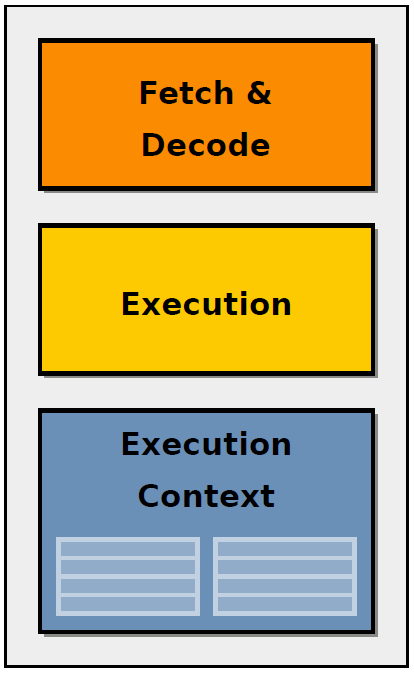
\includegraphics[height=0.25\paperheight]{CPU_Simple.png}
    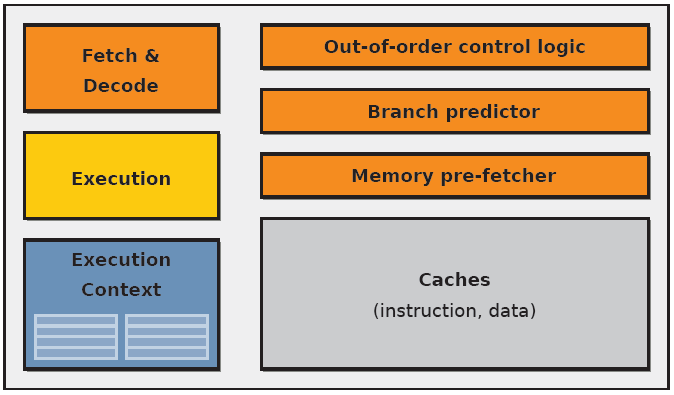
\includegraphics[height=0.25\paperheight]{CPU.png}
    \caption{Processor architecture diagrams. Left: A minimally functional processor. Right: A modern CPU. \cite{gpgpu}}
    \label{fig:cpu}
\end{figure}

This basic CPU design, however, has many speed limitations. Fetching instructions and data from main memory is an expensive operation and some of the execution units may spend time idle depending on the program flow. Many performance optimizations are used to reduce the impact of these limitations. Out-of-order execution allows instructions to be re-ordered to use execution units in parallel, memory is pre-fetched based on what data is expected to be needed by the next set of instructions, and the CPU will predict which branch will be taken by a program. These optimizations all improve the throughput offered by a single instruction stream.

Modern CPUs also take advantage of the knowledge that multiple instruction streams are all trying to execute simultaneously. If one stream stalls or does not fully utilize the execution units, the CPU will try to use idle units to begin calculations for an instruction set from a different stream. These changes, demonstrated in Figure \ref{fig:cpu}, facilitate higher performance for programs which separate programming instructions into multiple threads.

More recently, CPUs have moved to low levels of parallelization as well. Rather than increasing the speed of a single instruction stream, new models will duplicate hardware to support completely simultaneous execution of multiple instruction streams.

\subsection{GPU Architecture}

Due to the nature of computer graphics, GPUs were designed to focus on parallelization rather than single stream throughput. Graphical scenes are generally represented as a large number of discrete parts, each of which must be processed using a single transformation. These transforms can usually be applied to each discrete part independently of the rest of the scene. In order to process as many portions of the scene at once, a high number of basic processors is required \cite{gpgpu}.

GPUs require the same basic architecture as the CPU: a fetch and decode unit, an execution unit, and registers. Using this simple design does not provide the same throughput per stream as the more advanced CPU design, but it allows more processing cores to be included on the same chip to support many parallel streams. However, just as the CPU design became optimized for single streams, the GPU design was optimized for multiple streams.

Suppose we use an image editing program to change the hue of a picture with dimensions of 1280x1024. This picture has 1,310,720 individual pixels, each of which must be processed using the same linear transform. With a single core CPU this operation would need to be repeated for each of these pixels. If we use a GPU with 32 processing cores we could reduce the number of operations required to 40960.

Reducing the operations by using 32 processing cores is helpful, but would still be a slow process, particularly for more complicated transformations. Luckily, the GPU can optimize this operation further by taking advantage of the fact that each pixel is undergoing the same instructions. This optimization, demonstrated in Figure \ref{fig:simd} is called single instruction, multiple data (SIMD) processing. Rather than using a fetch and decode unit for every instruction stream, multiple registers and execution units share the same fetch and decode unit.

\begin{figure}
    \centering
	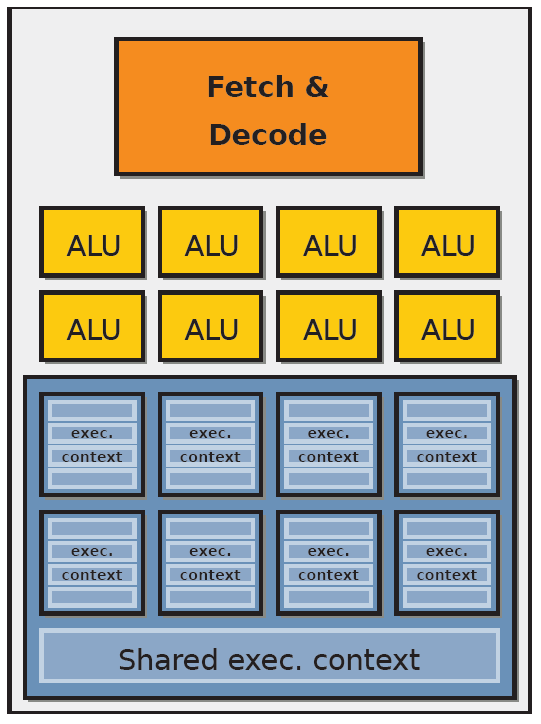
\includegraphics[height=0.25\paperheight]{SIMD.png}
    \caption{The SIMD architecture. \cite{gpgpu}}
	\label{fig:simd}
\end{figure}

Using SIMD processing the GPU is able to scale to very large number of simultaneous streams without requiring as much hardware. Now imagine that each of our 32 processing cores has 8 execution units and 8 registers. The calculation can now be completed in 5120 steps, a factor of 256 speedup! This performance boost does have one drawback: each of the processing cores must perform the same instruction across all execution units. This has some implications for GPGPU which will be discussed in the next section.

\subsection{Programming Model}

There are two main approaches to making the GPU's SIMD architecture available to programmers: explicitly using vector instructions, or implicitly using threads. Explicit instructions require the code to be written specifically for use on a GPU architecture. This can be beneficial as it requires the developer to carefully design algorithms for use on the GPU. However, manually writing highly parallelizable code can be difficult and hardware specific, thus reducing portability and requiring more development time \cite{gpgpu}.

Implicit models allow for programmers to write code as if it were for any multi-threaded CPU architecture. This can make the transition from CPU to GPU programming easier, but it also makes it easier to write very inefficient code. Despite the model allowing operations to be programmed using threads, groups of threads still must share the same fetch and decode unit. If the programmer is not aware of this limitation, it is possible to write code which attempts to branch threads operating on a single SIMD, lowering performance.

Unlike the CPU, the GPU does not have a sophisticated memory caching hierarchy. This is because graphical applications tend to share the same data across multiple execution units. Instead, the GPU memory architecture focuses on high bandwidth for transferring large amounts of data. As a result, random memory access suffers from high latency which can reduce performance. To overcome this problem for GPGPU solutions, a small cache of local memory is usually accessible. However, this cache is generally very small and so programmers are relied upon to write code that minimizes the need for random memory access.

In the early days of GPGPU, developers utilized the GPU by converting data input into graphical textures and defining algorithms in terms of programmable shaders. This was very difficult for some tasks which did not logically map well to graphics operations. In response, programming APIs have been developed to facilitate easier access to GPGPU. The two main APIs available today are CUDA, an nVidia specific API, and OpenCL, an open standard which is supported on both nVidia and AMD video cards \cite{gpgpu}.
